\subsection{Production Data Infrastructure}

While systems like PostGIS and QGIS are essential as exploration and debugging tools for GIS workflows, they suffer from important scale limitations that make them unsuitable for Machine Learning applications of the scope ultimately required by Vibrant Planet. To complement these systems, the team deployed a cloud infrastructure stack centered around a ``data lake'' architecture, consisting of the following components:
\begin{itemize}
  \item Amazon S3 as the data storage abstraction layer for both tabular and image data.
  \item A standalone Hive metastore, backed by a Postgres database, enabling the storage of tabular data.
  \item Trino as the distributed compute environment responsible for tabular data processing.
  \item Dask as the distributed compute environment responsible for image data processing.
\end{itemize}

The architecture stack was deployed using Kubernetes running on an Amazon EKS cluster. Dedicated node groups were set up for Trino (backed by T3.large instances) and Dask workers (backed by R5.large instances). Processing the area of interest required a peak of 30 instances running at any one time, with a total estimated run time for the entire data preparation pipeline of under 48 hours. Depending on its complexity, model training may add a significant amount of financial and time cost to these compute requirements. 

Image data processing was done using the same GDAL commands developed in the exploration stage, adapted using the pattern of ``embarassing parallelism'', where independent tasks were created for each of about 25,000 distinct image files identified in the area of interest. Hive tables were used to manage run metadata (i.e., what files needed processing, or had already been processed), whereas Dask workers were used to complete the processing itself. This design choice makes the processing incremental and easy to resume when faced with inevitable infrastructure errors.

\subsection{Data Pre-Processing}

The data processing consisted of the following concrete steps:

\begin{enumerate}
   \item \textbf{Identifying MGRS tiles of interest.} This task was done by leveraging an exhaustive listing of level 1B Sentinel data stored on Google Cloud Storage.\footnote{See: \url{https://cloud.google.com/storage/docs/public-datasets/sentinel-2#dataset_access}.} This table was imported into the data lake, as no similar metadata file was found for the Amazon instantiation of the Sentinel2 dataset. While the image listings themselves could not be used (due to Google's version of Sentinel2 containing only the ``rawer'' Level 1B data, as compared to the Level 2A data hosted by Amazon), the table proved useful due to its containing an exhaustive listing of all MGRS tiles for which Sentinel data is available, as well as their spatial coordinates. The identification of the 9 MGRS tiles of interest was thus done using a simple SQL filter query againstthis large metadata file. 
   \item \textbf{Identifying Sentinel data-takes of interest.} This was done simply by listing all existing data take files in the the S3 keys corresponding to each bucket.
   \item \textbf{Identifying high quality data takes.} This task involved reading the granule metadata corresponding to each datatake. Because the metadata lists an estimated cloud cover percentage, it was possible to separate out images with less than 35\% cloud cover. The 35\% threshold was identified during the exploratory phase.
   \item \textbf{Reprojecting Sentinel datatakes into a uniform coordinate system.} All Sentinel tiles are provided in the UTM coordinate system. Because the area of interest spans multiple UTM bands, it was necessary to harmonize them through reprojection into the California Albers projection -- a planar coordinate system developed specifically for geographic information relating to state's geography.
   \item \textbf{Clipping reprojected datatakes to uniform grid.} Because datatakes corresponding to multiple MGRS tiles could cover the same area, it was necessary to overlay them to create a composite dataset. The first step in creating the overlay involved clipping each tile to a uniform extent, using square tiles with a side of 40km (this choice was dictated by memory constraints on individual machines used for the data processing.)
   \item \textbf{Merging clipped datatakes into annual summaries.} Clipped datatakes corresponding to the same grid square and year were merged using a simple noise reduction algorithm. Namely, a median value was taken for each pixel across all datatakes referring to the same location during each year's dry season (to minimize artifacts due to snow and clouds, given that clouds were not removed from the processed images.). Where more than 18 data takes were present, the median was approximated as the median of median values taken across each batch of up to 18 data takes (the batch size was determined empirically, to fit within memory constraints.)
\end{enumerate}

The pre-processing results in a composite image for each band and for each year. This image, an example of which is shown below, represents one layer of features for the Machine Learning model.

\begin{figure}
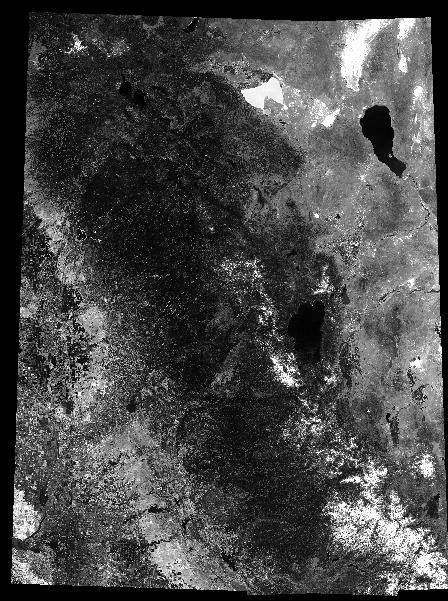
\includegraphics[width=\textwidth]{images/band.png}
\end{figure}

